\chapter{Anhang}
\appendix
	\section{Begriffsdefinitionen}

	\section{Abkürzungsverzeichnis}
		\begin{acronym} 
			% Acronym mit \acro hinzu
			\acro{API}{Application Programming Interface (Programmierschnittstelle)}
			\acro{Add-On}{Erweiterungspaket}
			\acro{JRE}{Java Runtime Environement}
			\acro{JSON}{JavaScript Object Notation}
			\acro{HTTP}{Hypertext Transfer Protocol}
		\end{acronym}
	
	% Abbildungsverzeichnis
	\listoffigures
	
	\section{Aufwandsabschätzung}
	%Aufwandsabschätzungstabelle einfügen

	\begin{figure}
		\centering
		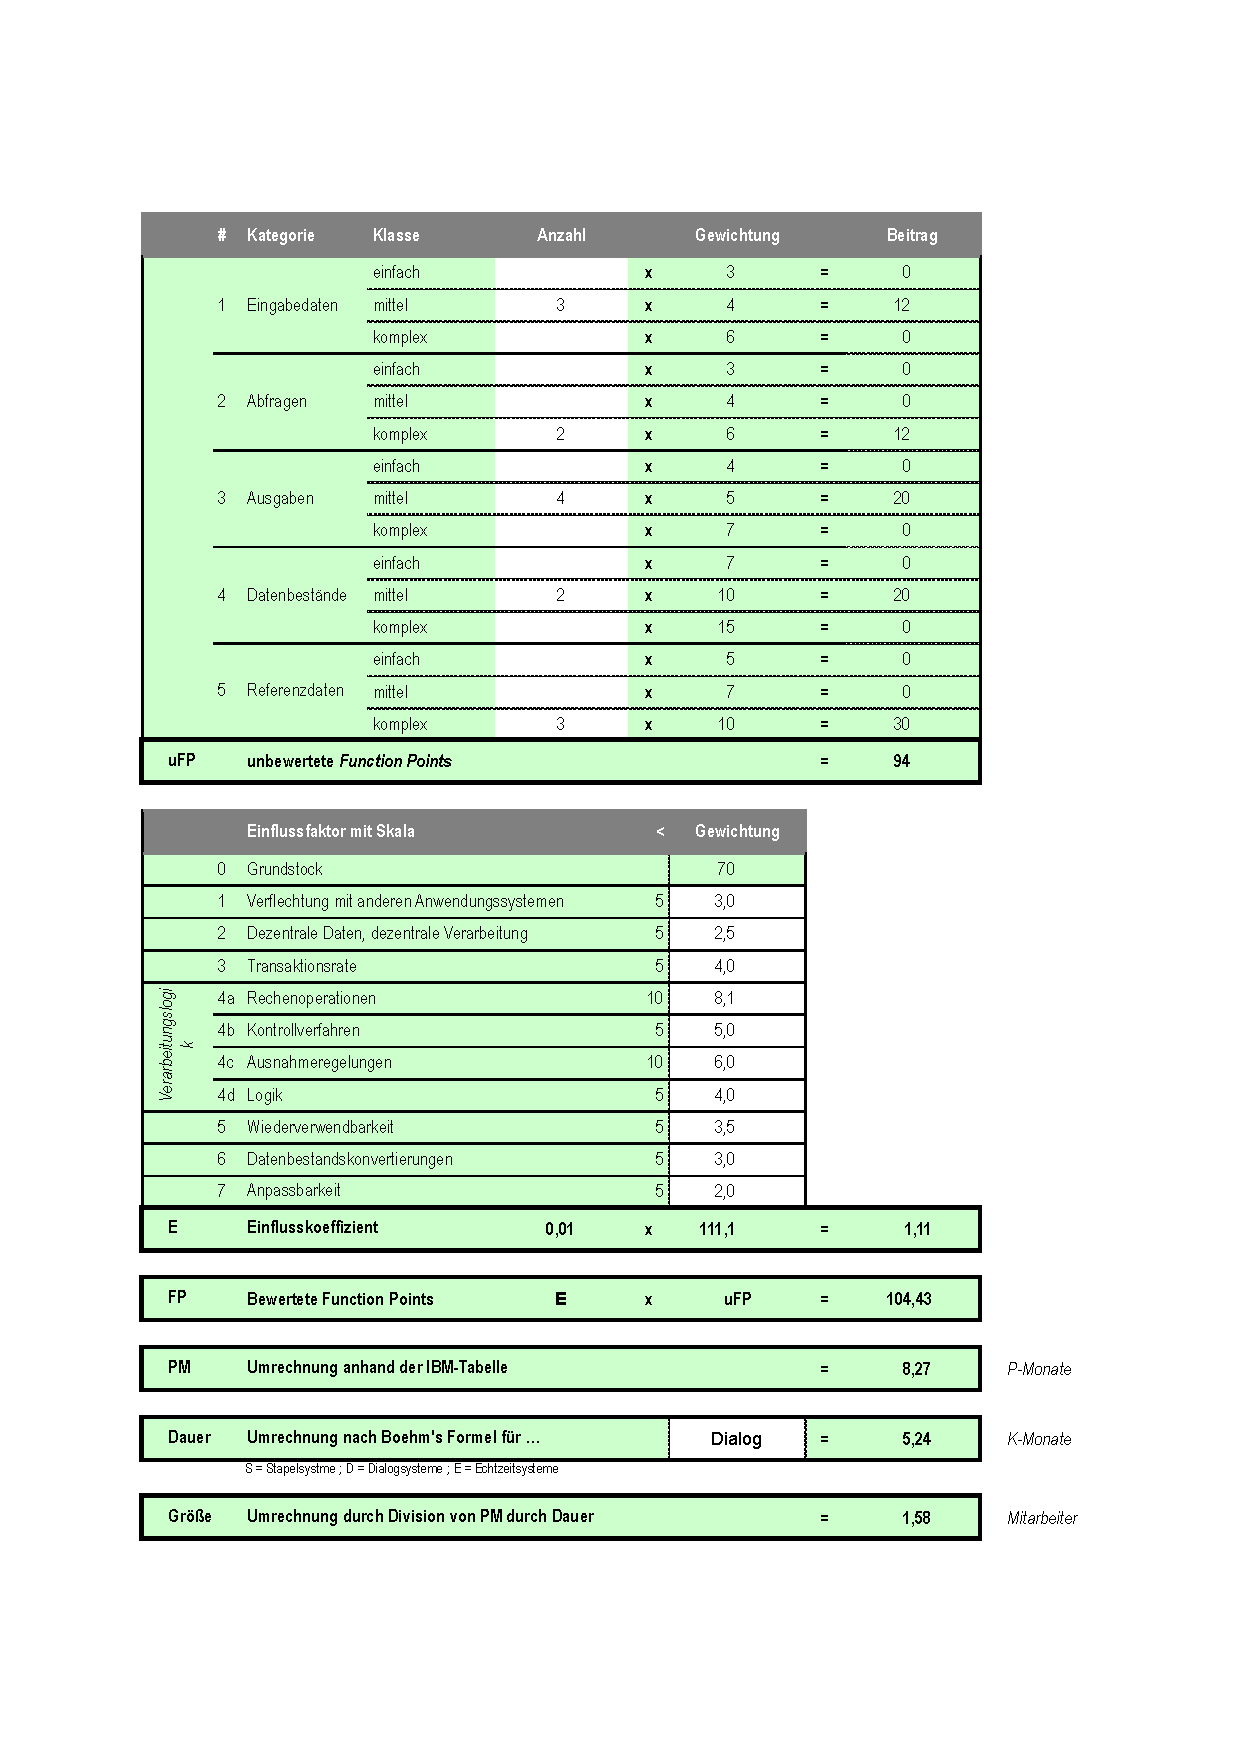
\includegraphics[width=0.9\textwidth]{data/Aufwandsabschaetzung.pdf}
		\caption{Aufwandsabschätzungen}
	\end{figure}
	
	\section{Datenflussdiagramme sowie weitere Diagramme}

	\begin{figure}[H]
		\centering
		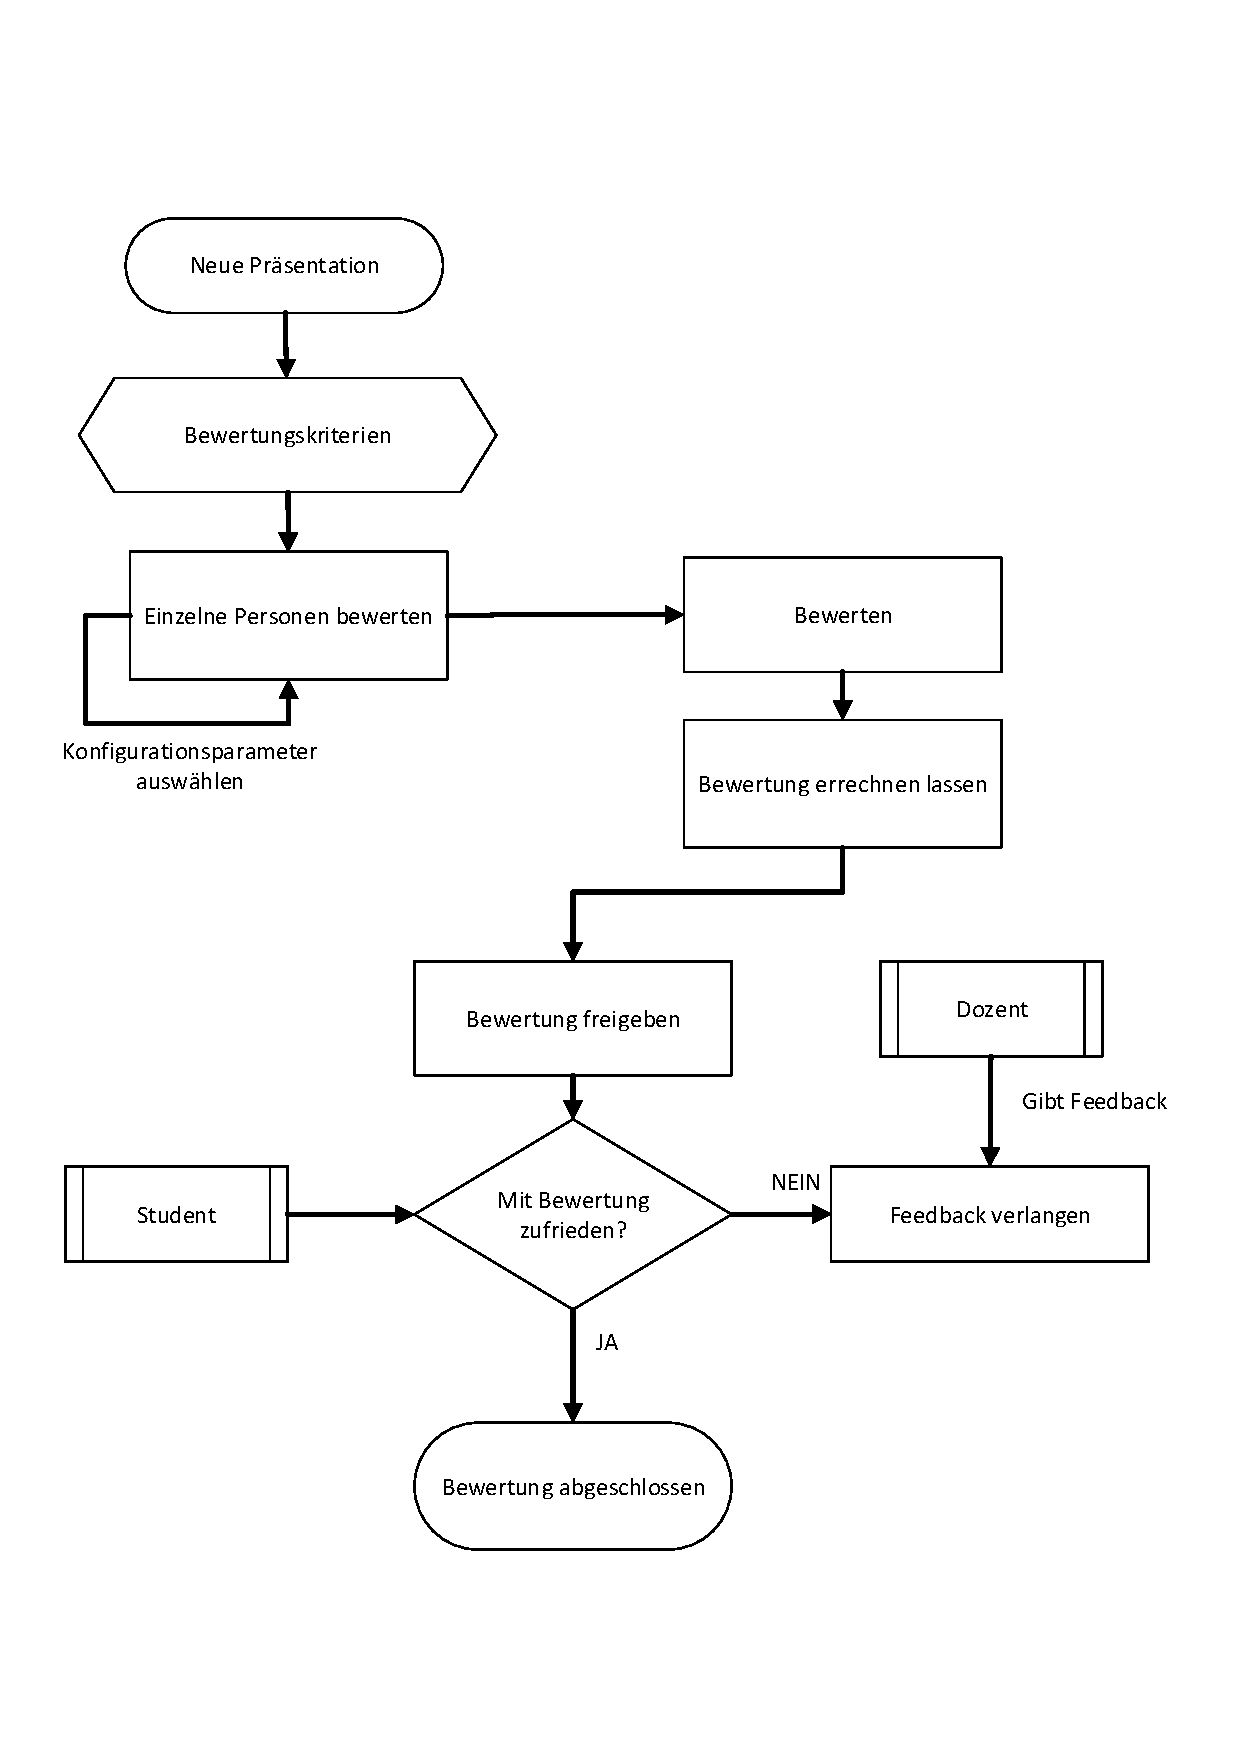
\includegraphics[height=0.9\textheight]{../Diagramme/Beispiel-FlussdiagrPraesi.pdf}
		\caption{Beispielprozess einer Bewertung einer Präsentation}
	\end{figure}
	\begin{figure}[H]
		\centering
		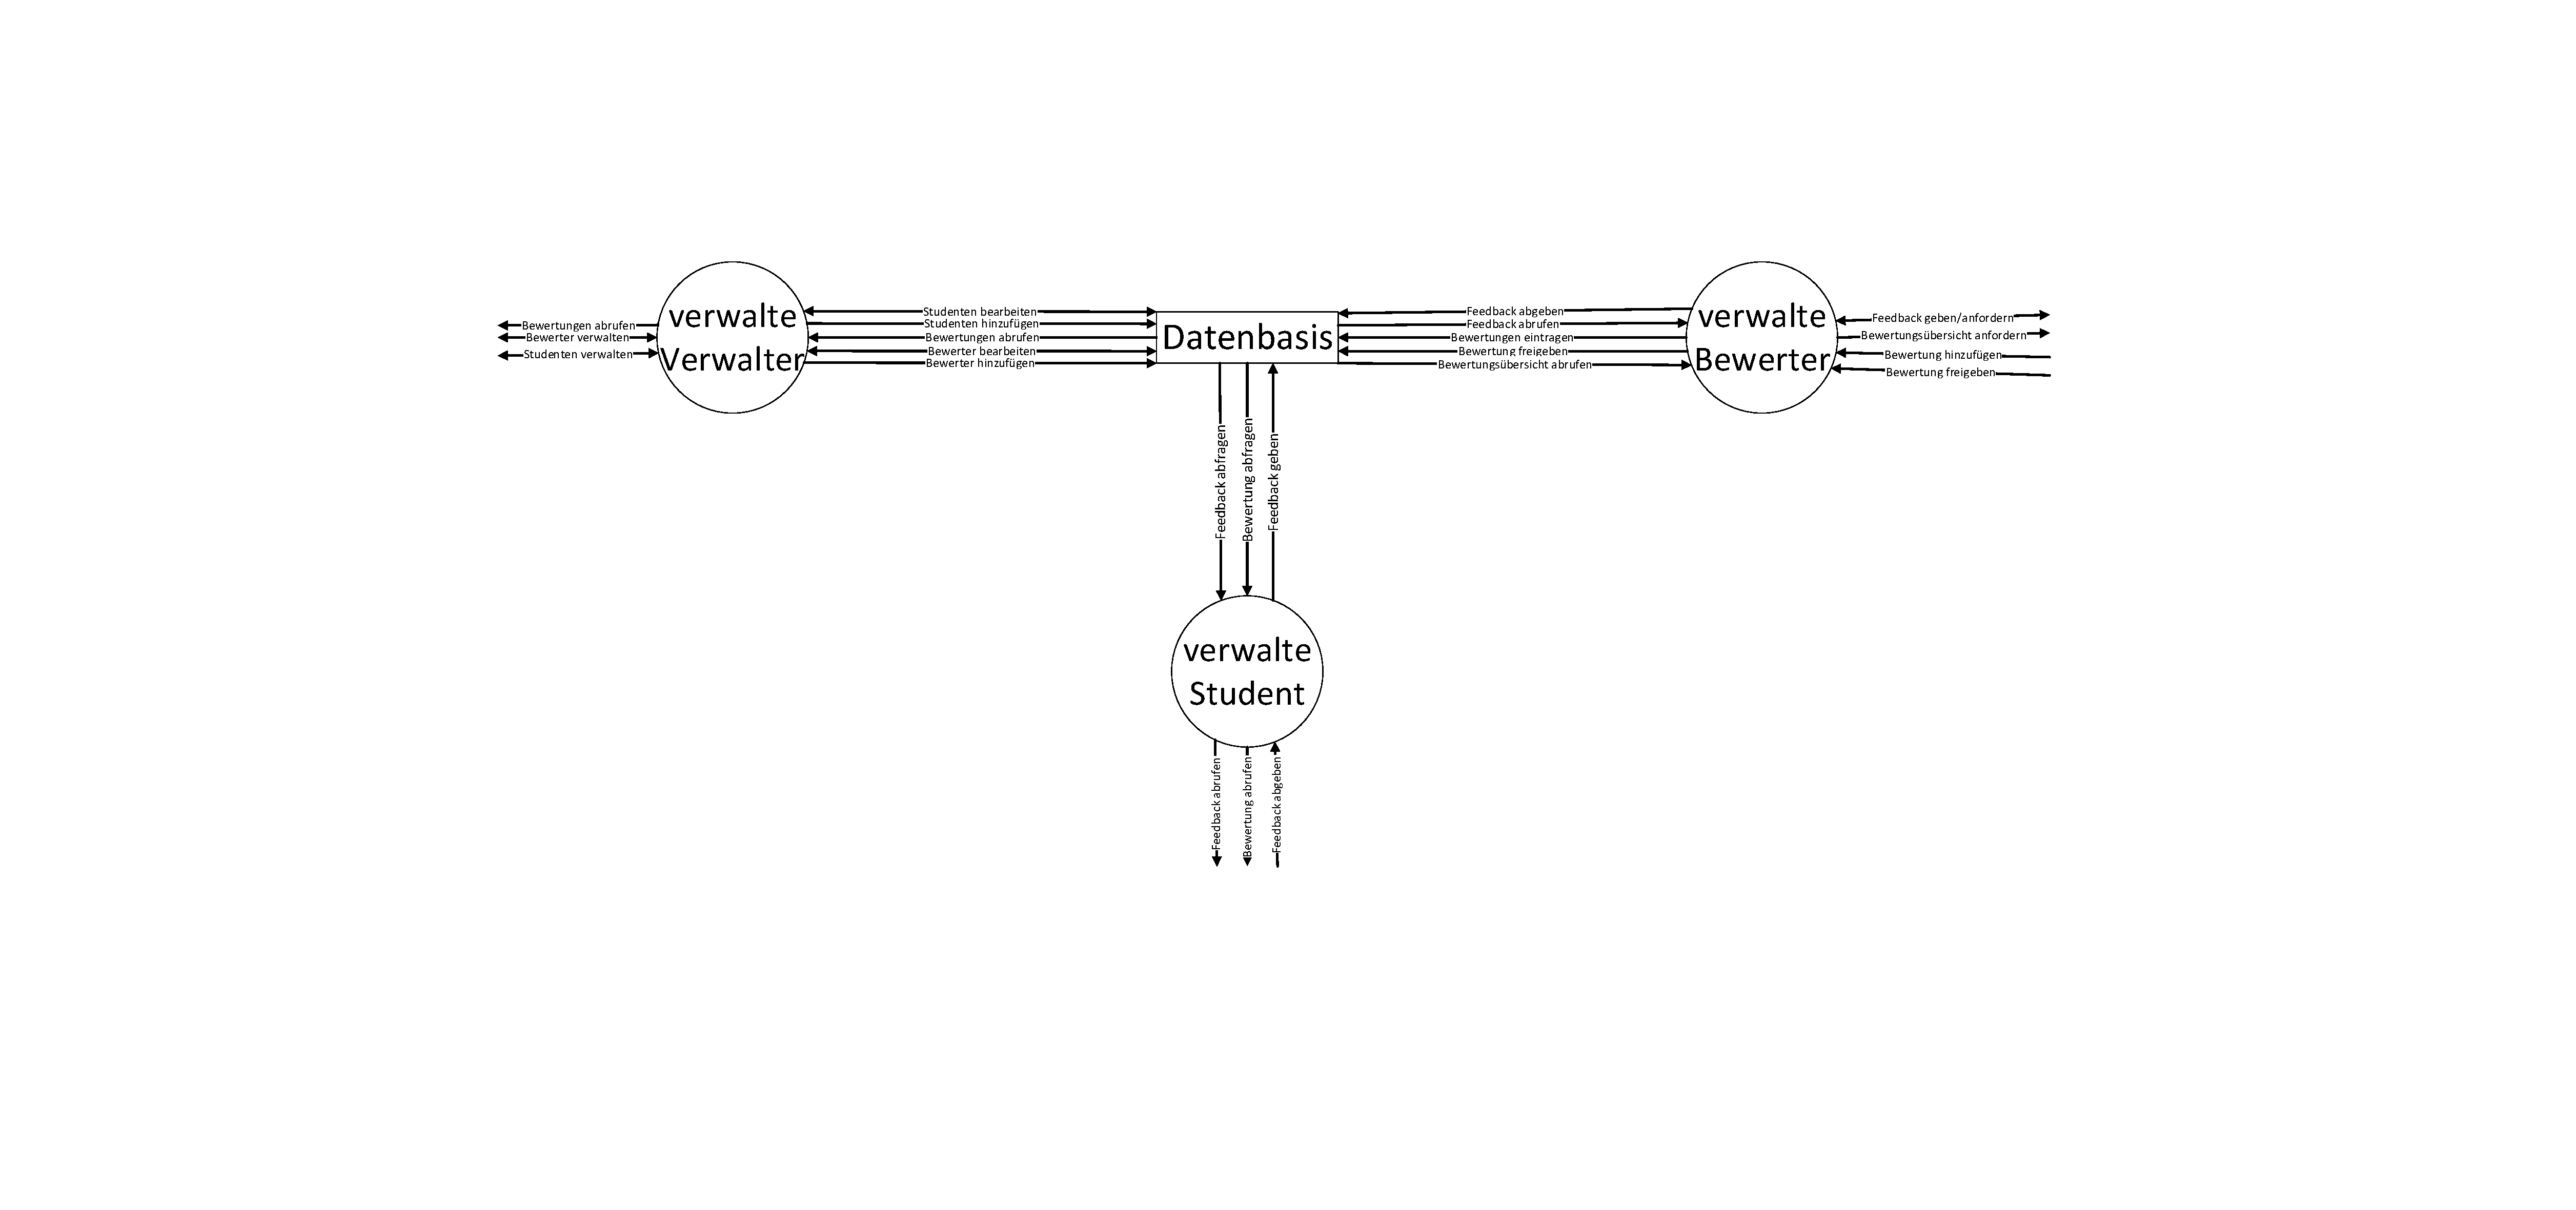
\includegraphics[width=1.4\textwidth, angle=90, origin=c]{../Diagramme/Kontextdiagramm_DFD0.pdf}
		\caption{Kontextdiagramm}
	\end{figure}
	\begin{figure}[H]
		\centering
		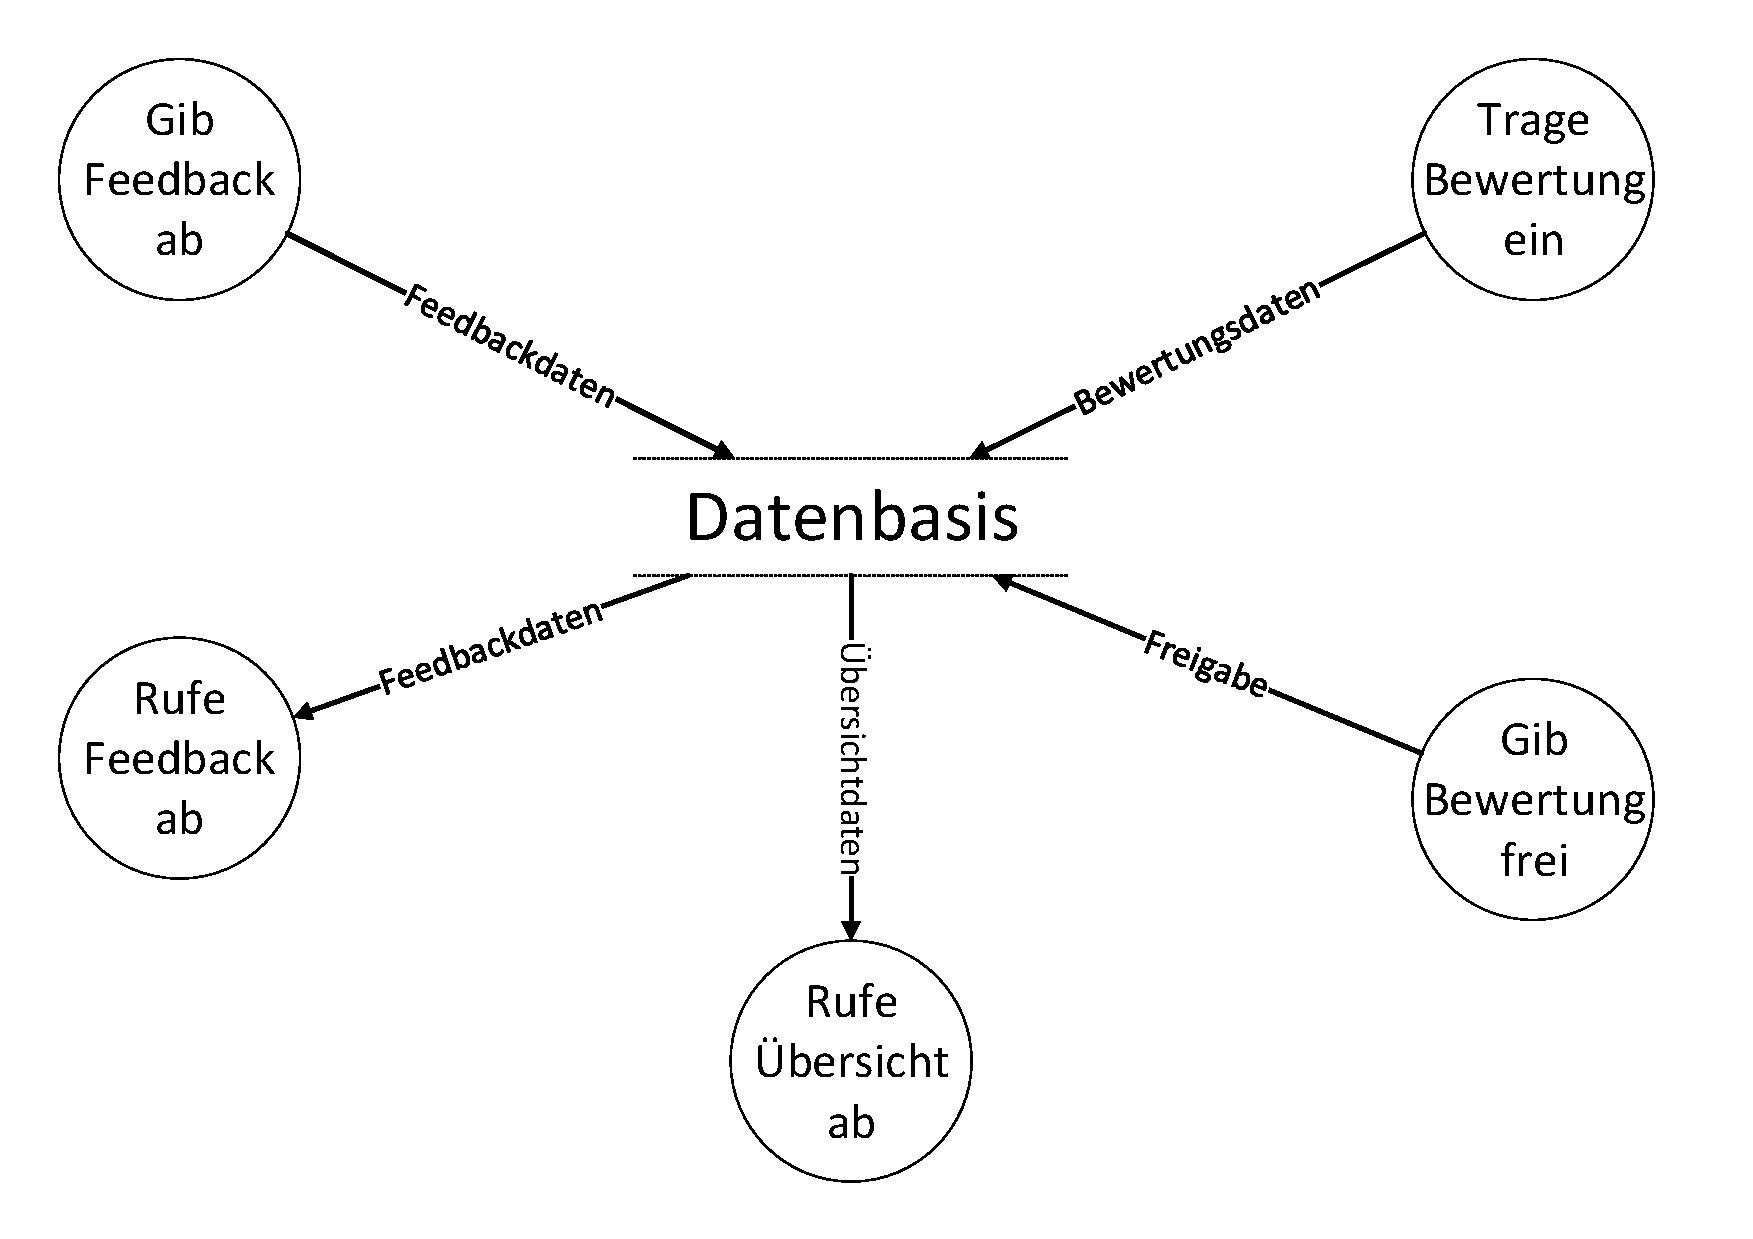
\includegraphics[width=1.4\textwidth, angle=90, origin=c]{../Diagramme/Kontextdiagramm_DFD2_Bewerter.pdf}
		\caption{Datenflussdiagramm Bewerter}
	\end{figure}
	\begin{figure}[H]
		\centering
		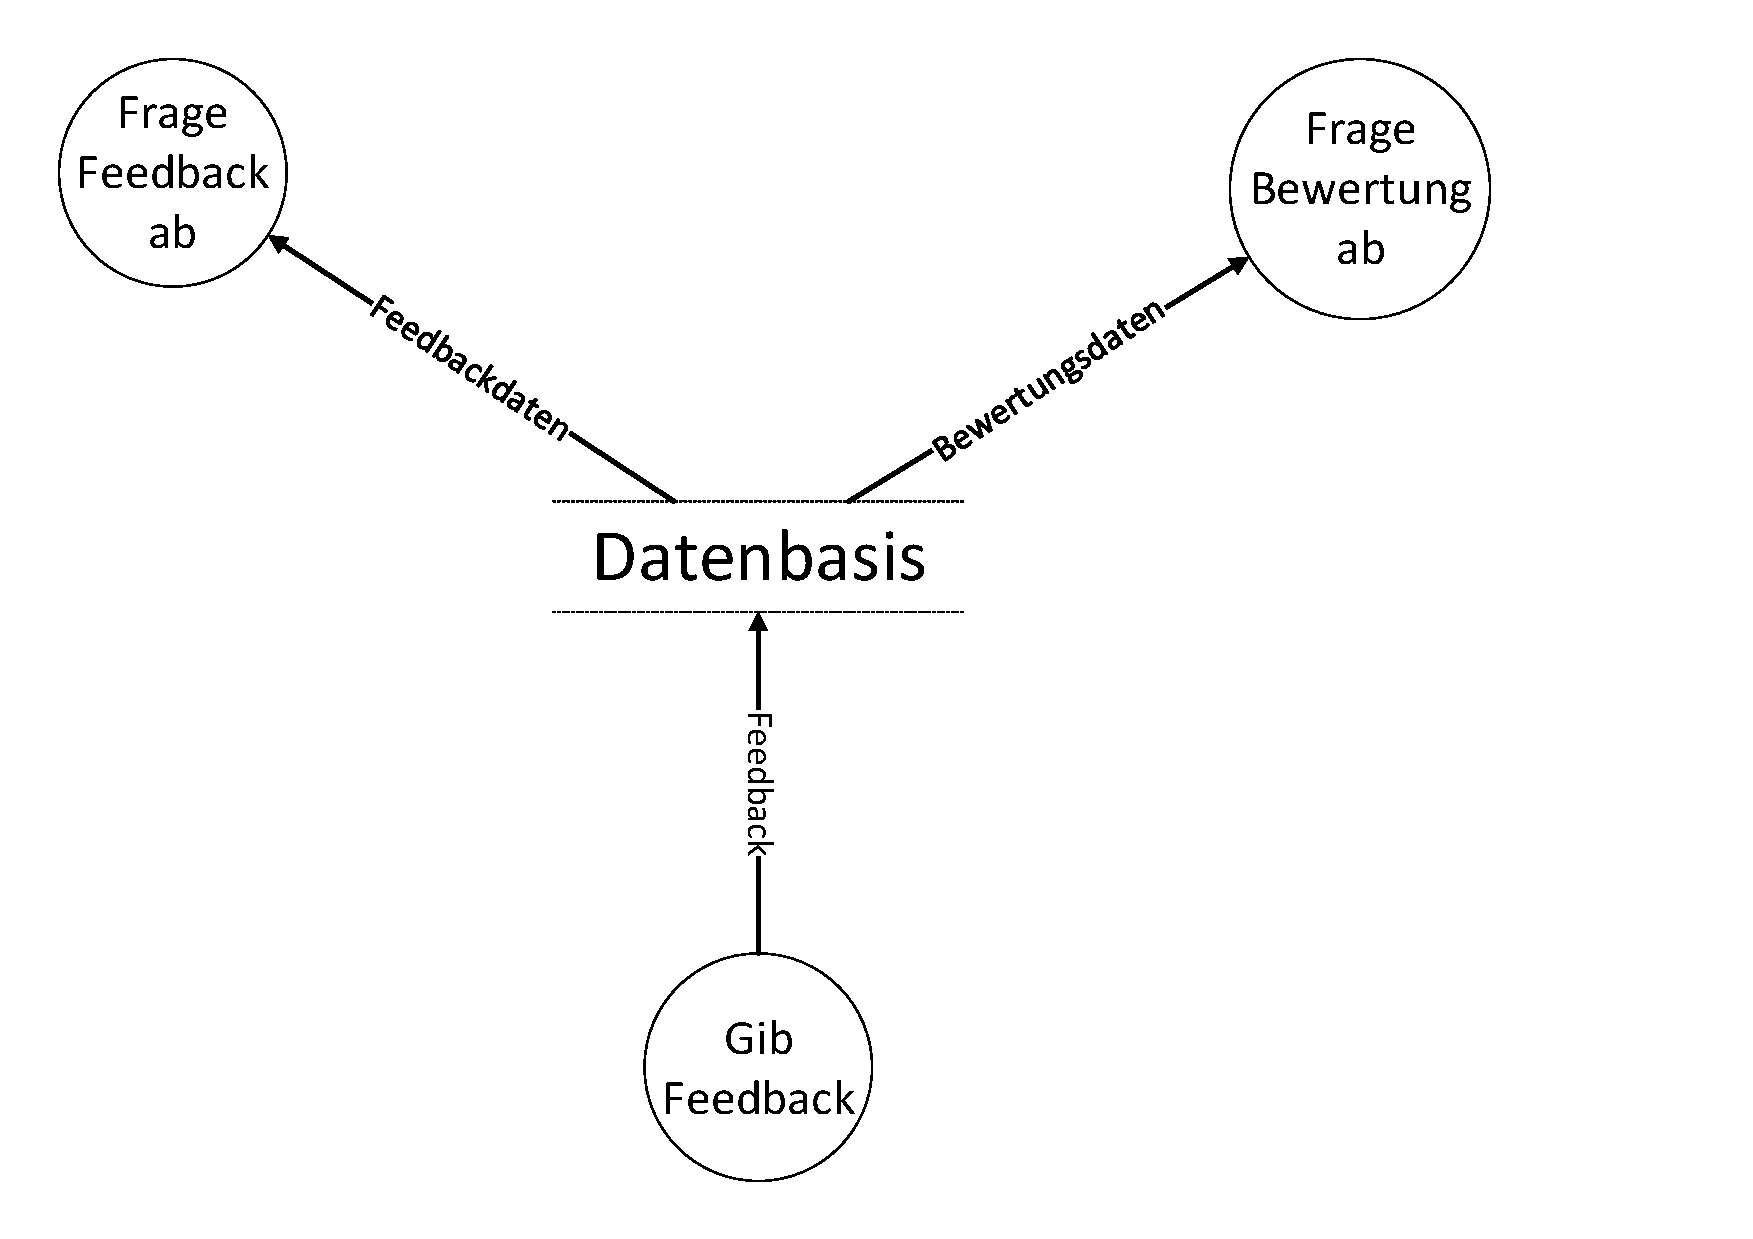
\includegraphics[width=1.4\textwidth, angle=90, origin=c]{../Diagramme/Kontextdiagramm_DFD2_Student.pdf}
		\caption{Datenflussdiagramm Student}
	\end{figure}
	\begin{figure}[H]
		\centering
		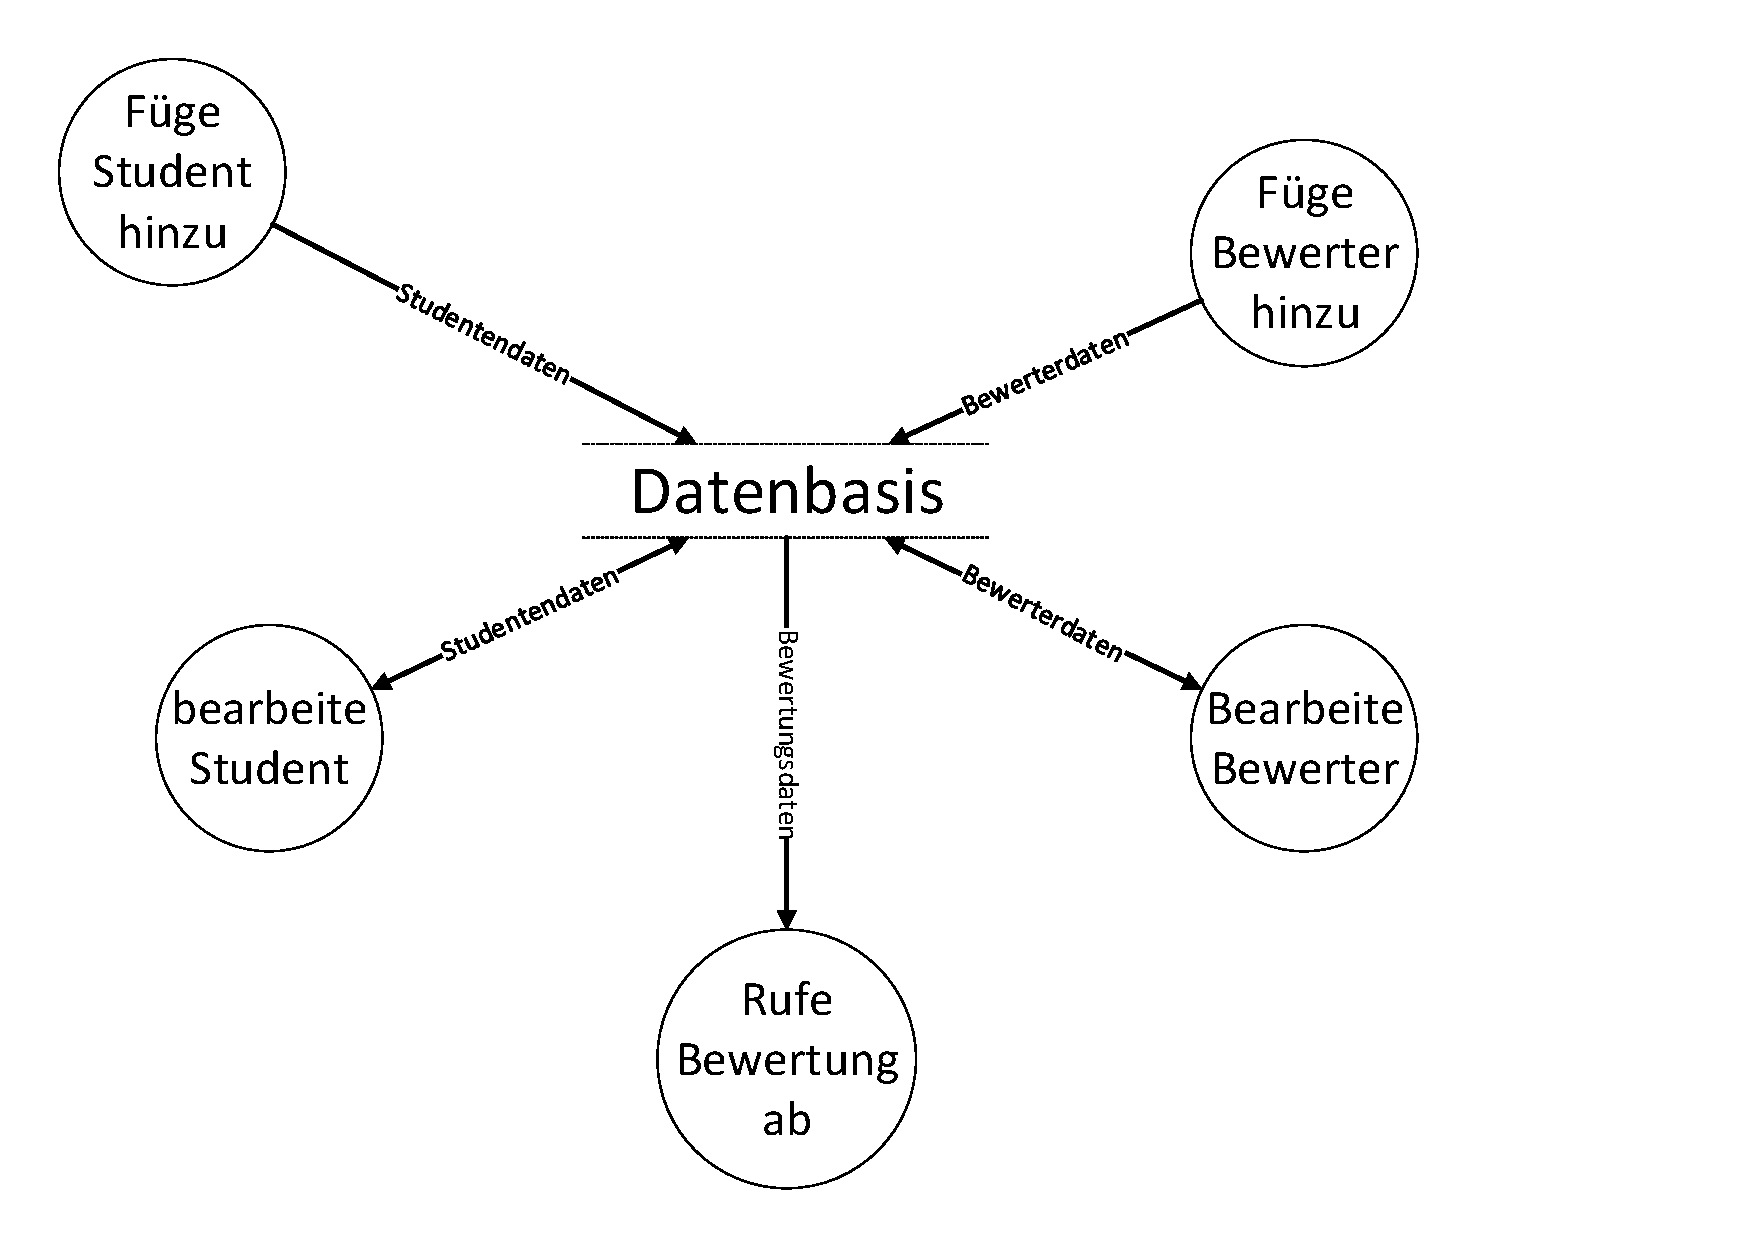
\includegraphics[width=1.4\textwidth, angle=90, origin=c]{../Diagramme/Kontextdiagramm_DFD2_Verwalter.pdf}
		\caption{Datenflussdiagramm Student}
	\end{figure}
	
	
	\listoftables